\section{Application pratique}

On applique l'analyse par composantes principales et l'analyse par composantes principales avec noyau sur le jeu de données MNIST. Une donnée représente l'intensité de gris entre 0 et 255 des 728 pixels d'un image 28$\times$ 28 de chiffres entre 0 et 9. Elles ont été récoltées par \cite{lecun1998gradient}. Voici un exemple des données : 

\begin{figure}[H]
	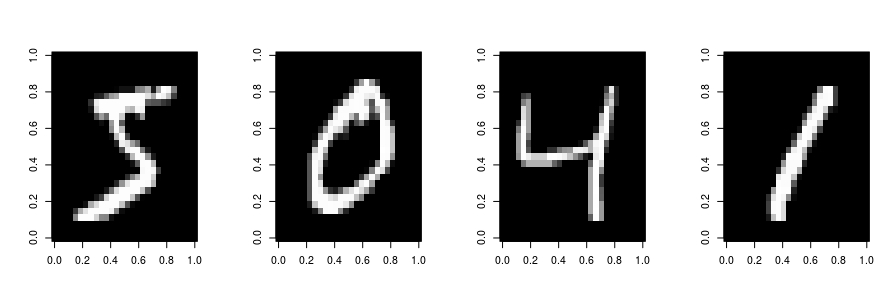
\includegraphics[width=\textwidth]{digits-original}
	\caption{4 premiers exemples de MNIST}
	\label{fig:mnist-original}
\end{figure}

On créer aussi un jeu de données modifié de MNIST, où un applique un bruit gaussien. Voici les mêmes exemples que dans la figure \ref{fig:mnist-original} :

\begin{figure}[H]
	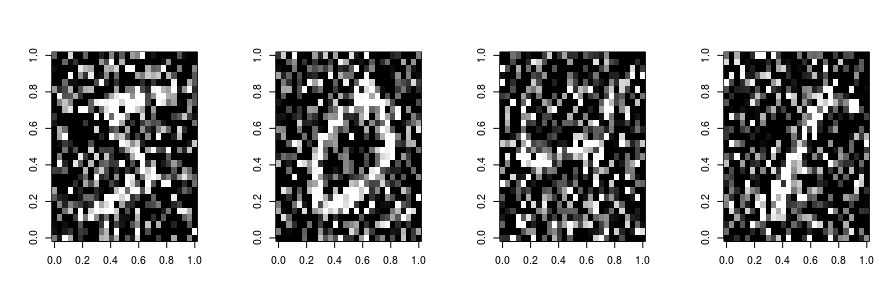
\includegraphics[width=\textwidth]{digits-noisy}
	\caption{4 premier exemples de MNIST avec bruit gaussien}
\end{figure}

Une analyse par composantes principales est identique à une analyse par composantes principales avec un noyau linéaire. On projète les données selon les deux premières composantes principales. On obtient

\begin{figure}[H]
	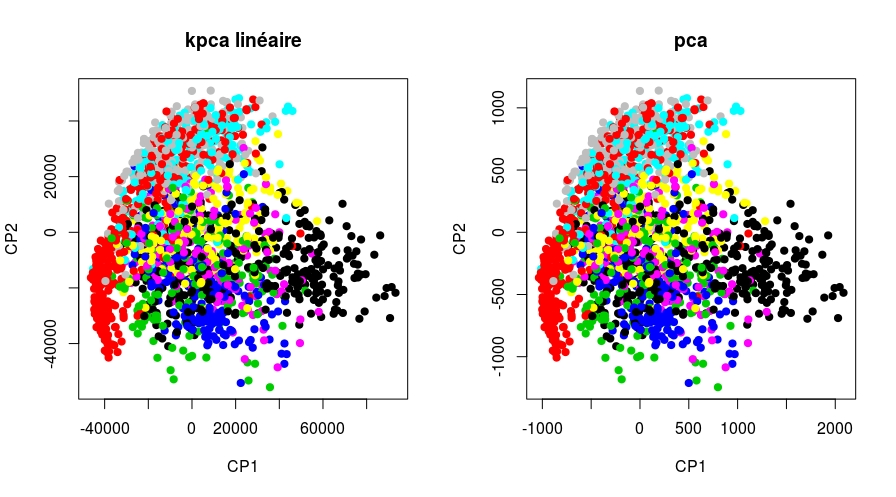
\includegraphics[width=\textwidth]{comparaison-lineaire}
\end{figure}

Il n'y a pas de flexibilité à cette méthode. On remplace la matrice variance-covariance par différents noyaux et on présente les projections dans la prochaine figure. 

\begin{figure}[H]
	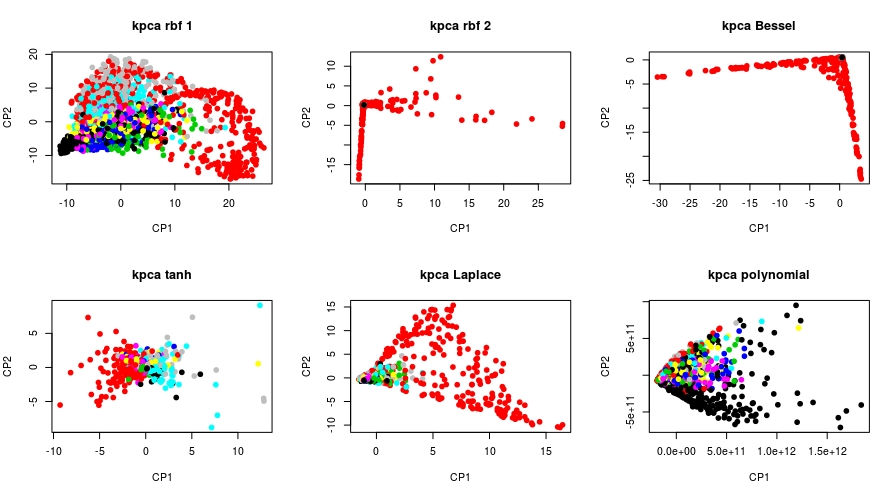
\includegraphics[width=\textwidth]{comparaison-kernel}
	\caption{Projection des deux premières composantes principales selon différents noyaux.}
\end{figure}

On remarque que le choix du noyau a beaucoup d'importance sur la projection. Les données en rouge représentent le chiffre 1 et la plupart des noyaux peuvent séparrer les données. Le noyau polynomial est performant pour segmenter les chiffres 0. 

On applique ensuite kACP sur les données MNIST bruitées. On obtient 

\begin{figure}[H]
	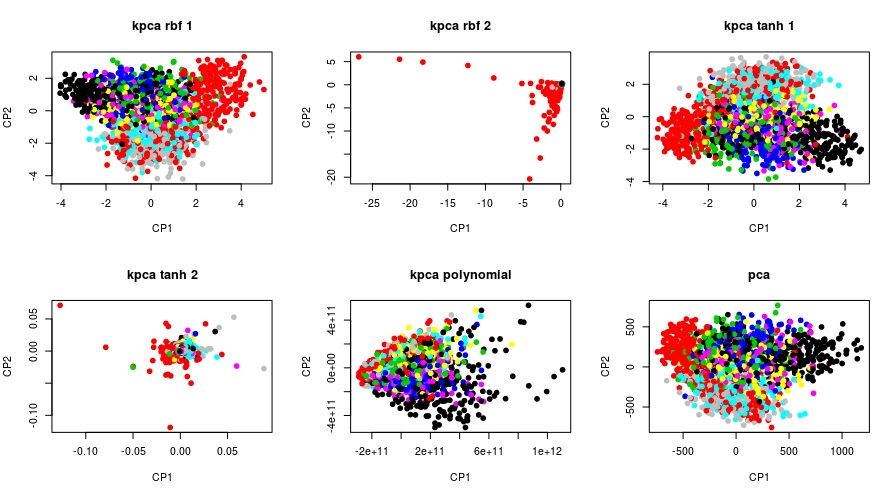
\includegraphics[width=\textwidth]{comparaison-noisy}
	\caption{Projection des deux premières CPs selon différents noyaux.}
\end{figure}

On remarque que certains noyaux sont moins performants pour capturer l'information que sans le bruit, mais que certains sont capables de trouver les relations non-linéaires dans les données bruitées pour retrouver l'information originale. 
